

\section{Motifs}

In this chapter we analyze the strucarl. The term motif referes
to... . Studies of \textcite{Song2005} and \textcite{Perin2011} show
stuff.

\subsection*{Three-neuron patterns}

Song motifs:


\begin{figure}[H]
  \centering
  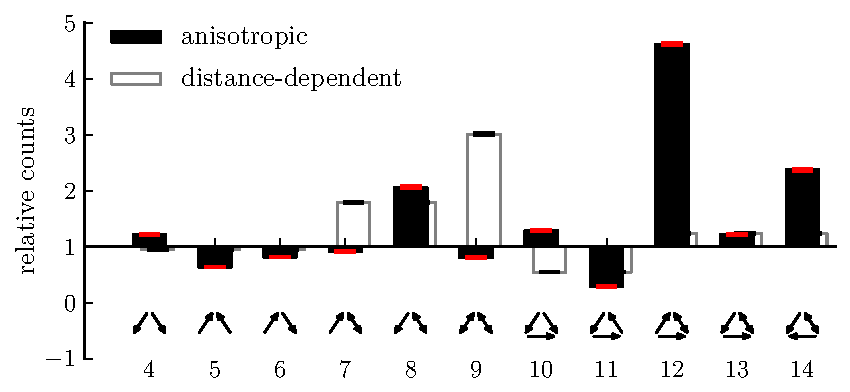
\includegraphics[width=0.95\linewidth]{%
    plots/4839ce41_aniso_dist.pdf} 
  \captionsetup{skip=8pt}
  \caption{\textbf{Relative occurrence of three-neuron patterns}
    Extracting the counts of three-node motifs in anisotropic (filled
    bars) and distance-dependent networks (unfilled bars), the
    quotient of the obtained count with the number of occurrences
    expected from the two-neuron connection probabilities in the
    networks (rs =, ,, cf.) shows the over- and underrepresentation of
    specific motifs in the network (red and black errorbars are
    SEM). In anisotropic networks pattern number \enquote{12}, for
    example, appears around five times more often than we would expect
    from the occurrence two-neuron connections. The relative counts
    for anisotropic networks resemble the findings of
    \textcite{Song2005} and differ significantly from the counts in
    distance-dependent networks, implying that anisotropy has a strong
    influence on the relative occurrence of three-neuron
    patterns. (\smtcite{4839ce41}) }
  \label{fig:distance_theory_compare}
\end{figure}



\begin{figure}[H]
  \centering
  \renewcommand{\tabcolsep}{0pt}
  \setlength\extrarowheight{0pt}
  \begin{tabular}{ll}
    \begin{overpic}[width=0.5\textwidth]{%
        /users/hoffmann/research/cn_k_test.pdf}
      %\put(12,56){\small $\eta = 0$}
    \end{overpic}
    &
    \begin{overpic}[width=0.5\textwidth]{%
        /users/hoffmann/research/cn_k_test.pdf}
      %\put(12,56){\small $\eta = 0.25$}
    \end{overpic}
    \\
    \begin{overpic}[width=0.5\textwidth]{%
        /users/hoffmann/research/cn_k_test.pdf}
      %\put(12,56){\small $\eta = 0.5$}
    \end{overpic}
    &
    \begin{overpic}[width=0.5\textwidth]{%
        /users/hoffmann/research/cn_k_test.pdf}
      % \put(12,56){\small $\eta = 0.75$}
      %\put(4,-4){\small$0$}\put(78,-4){\small$200$}
    \end{overpic}
    \\
    % \begin{overpic}[width=0.28\textwidth]{%
    %     plots/77995b6b_in100.pdf}
    %   \put(12,56){\small $\eta = 1$}
    %   \put(4,-4){\small$0$}\put(78,-4){\small$200$}
    % \end{overpic}
    % & 
    % \begin{overpic}[width=0.28\textwidth]{%
    %     plots/77995b6b_indst.pdf}
    %   \put(12,56){\small distance}
    %   \put(4,-4){\small$0$}\put(78,-4){\small$200$}
    % \end{overpic}
    % \\
  \end{tabular}
  \caption{\textbf{In-degaree distrbution not affected by varying
      degrees of anisotropy} 
    (\smtcite{77995b6b}). }
  \label{fig:in_degree_rewiring}
\end{figure}



%%% Local Variables: 
%%% mode: latex
%%% TeX-master: "../dplths_document"
%%% End: 
